% !TEX root=talk.tex
\section{Antecedentes}

\begin{frame}
\frametitle{Definiciones}
Una \emph{gráfica geométrica} $\mathsf{G}=(V,E)$ es un par de conjuntos $V$ de puntos en el plano y $E$ de 
segmentos de recta que unen pares de puntos de $V$. Llamamos vértices y aristas a estos conjuntos,
respectivamente. Una gráfica geométrica es \emph{completa} si contiene a todas las 
aristas entre pares de vértices de $V$.
\begin{figure}
	\centering
	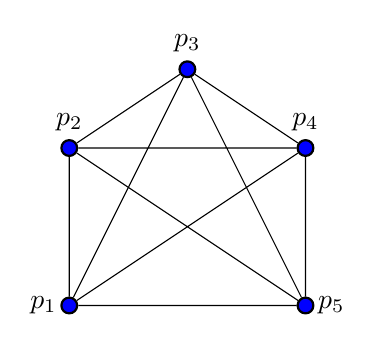
\begin{tikzpicture}
	\begin{scope}[every node/.style={circle,thick,draw,fill=blue,minimum size=2mm,inner sep=0pt}]
	    \node[label=left:{$p_1$}] (p1) at (0,0){};
	    \node[label={$p_2$}] (p2) at (0,2){};
	    \node[label={$p_3$}] (p3) at (1.5,3){};
	    \node[label={$p_4$}] (p4) at (3,2) {};
	    \node[label=right:{$p_5$}] (p5) at (3,0) {};
	\end{scope}
	\draw \foreach \k [count=\j from 1] in {1,...,5}
		\foreach \kk in {\j,...,5}
			{(p\k)--(p\kk)};
	\end{tikzpicture}
	\caption{En esta gráfica geométrica $V=\{p_1,p_2,p_3,p_4,p_5\}$ y $E=\{(p_1,p_2),(p_1,p_3),\dots,(p_4,p_5)\}			$. Esta gráfica geométrica es completa.}
\end{figure}
\end{frame}